\section{Die alljährliche Nikolaus-Aktion der Fachschaft Physik}
\begin{multicols}{2}
\textbf{HOHOHO, von drauß' vom Walde komm ich her\dots\
	mit Schokolade, was will man mehr?}

Wie jedes Jahr in der Vorweihnachtszeit habt ihr pünktlich zum Nikolaustag die Möglichkeit euren Kommilitonen eine süße Freude zu bereiten, genauer gesagt könnt ihr ihnen einen Schokonikolaus mit Grußkärtchen schenken. 
Die Nikoläuse werden dann \leftqq stilecht\rightqq  vom Nikolaus (oder eher Weihnachtsmann) und Engeln in den Grundvorlesungen verteilt.

Wozu das ganze? Ihr habt die perfekte Möglichkeit, besonderen Menschen zu zeigen, dass ihr sie mögt. Oder alternativ auch als Dankeschön für abgeschriebene Übungsaufgaben, als Motivationshilfe, 
unauffälliger Flirtversuch oder um die Vorlesung für eine Weile zu unterbrechen. Es wurde auch schon versucht, Professoren bzgl.\ der Übungszettel/Klausuren zu bestechen. 
Jedoch wurde bis dato keine signifikante Auswirkung gemessen. Man munkelt aber, dass vereinzelte Grußkärtchen in den Büros der Profs aufzufinden sind und dort stetig zu einer guten Laune beitragen ;)

Die Nikolaus-Aktion wird immer rechtzeitig vorher in den Vorlesungen angekündigt. So habt ihr die Möglichkeit einige Tage vorm Nikolaustag in der Fachschaft euer Grußkärtchen zu erwerben und kreativ zu gestalten. 
Das fertige Kärtchen muss nur in der Fachschaft abgegeben werden und um den Rest kümmern wir uns ;)

Verteilt werden die Nikoläuse am 6.~Dezember in den jeweiligen Pflichtmodule des ersten, dritten und fünften Semesters. Das bedeutet entweder in der Mathe- oder Physik-Vorlesungen (je nachdem, welche gerade an dem besagten Tag ist).
2-Fach-Bachelor-Studenten müssen ein wenig aufpassen, wenn die Nikoläuse in einer Mathe-Vorlesungen verteilt werden.
Sollte die beschenkte Person nicht in der Vorlesung anwesend sein, kann sie den Nikolaus noch einige Tage im Raum der Fachschaft abholen.
Fällt der 6.~Dezember aufs Wochenende, werden die Nikoläuse am folgenden Vorlesungstag von uns ausgeteilt.

Auf eine schöne Vorweihnachtszeit, euer Nikolausteam!

\fibelsig{Miriam N.}
\end{multicols}

\vspace{\fill}
\begin{center}
	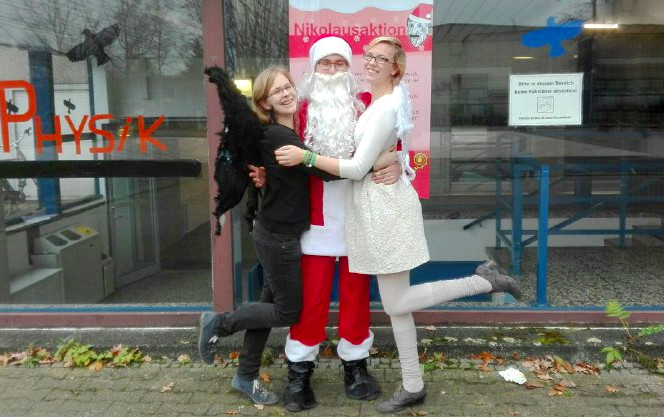
\includegraphics[width=0.99\textwidth]{res/nikolaus.jpg}
\end{center}
